\documentclass[12pt,twoside,titlepage]{ingenius}
\usepackage[figuresright]{rotating}
\usepackage{adjustbox}
\usepackage{units}
\usepackage{dblfloatfix}
\usepackage{amssymb}
\usepackage{caption}
\usepackage{subcaption}
\usepackage{bm}
\usepackage{textcomp}
\usepackage{pifont}
\usepackage{cite}
\usepackage{xcolor,colortbl}
\usepackage{amsmath}
\usepackage{upgreek}
\usepackage{graphicx}
\usepackage{tikz}
\usepackage{pifont}
\usetikzlibrary{shapes,arrows}
\usepackage{textcomp}
\usepackage{multirow}
\usepackage{float}
\usepackage{soul}
\usepackage{rotating}
\usepackage{hyperref}
\usepackage{booktabs}
\usepackage{enumitem}
\graphicspath{{figures/}}
%===========================================
%========
\usepackage{tikz,xcolor,hyperref}
% Make Orcid icon
\definecolor{lime}{HTML}{A6CE39}
\DeclareRobustCommand{\orcidicon}{%
	\begin{tikzpicture}
	\draw[lime, fill=lime] (0,0) 
	circle [radius=0.16] 
	node[white] {{\fontfamily{qag}\selectfont \tiny ID}};
	\draw[white, fill=white] (-0.0625,0.095) 
	circle [radius=0.007];
	\end{tikzpicture}
	\hspace{-2mm}
}
\foreach \x in {A, ..., Z}{%
	\expandafter\xdef\csname orcid\x\endcsname{\noexpand\href{https://orcid.org/\csname orcidauthor\x\endcsname}{\noexpand\orcidicon}}
}
%========================================================
\titulo{Retrofitting IoT para un laboratorio remoto de cinemática en ingeniería: diseño, implementación y validación técnica de un prototipo para el estudio del MRUA en un entorno de aprendizaje híbrido}
\tituloa{IoT Retrofitting for a Remote Kinematics Laboratory in Engineering: Design, Implementation, and Technical Validation of a Prototype for the Study of UARM in a Hybrid Learning Environment}
%========================================================
\newcommand{\orcidauthorA}{0009-0003-6240-3462}
\newcommand{\orcidauthorB}{0000-0001-5628-3351}
\autores{Walter Santiago Sosa Mejía $^{1}$,\orcidA{} Manuel Rogelio Nevàrez Toledo $^{1,}$*\orcidB{}}
\adscripcionautor{%
$^{1}$ \quad Pontificia Universidad Cat\'olica del Ecuador, Sede Esmeraldas, Esmeraldas, Ecuador; wssosa@pucese.edu.ec (W.S.S.M.); manuel.nevarez@pucese.edu.ec (M.R.N.T.)\\
* Autor de correspondencia / Corresponding author: manuel.nevarez@pucese.edu.ec}

%%Datos para referencias
\newcommand{\apellido}{Sosa Mejía et al.}% Apellido o apellidos para referencia 
\newcommand{\titu}{IoT Retrofitting for a Remote Kinematics Laboratory}%titulo a la referencia
\newcommand{\tipo}{Art\'iculo Cient\'if{}ico / Scientif{}ic Paper} 
%========================================================
%%Datos para propiedades del pdf no requiere ser llenado
\newcommand{\autor}{Walter Santiago Sosa Mejía, Manuel Rogelio Nevàrez Toledo}%autor para propiedades del pdf
\newcommand{\pc}{Retrofitting, Internet de las Cosas, Laboratorios remotos, MRUA}%palabras clave para propiedades del pdf
\newcommand{\kw}{Retrofitting, Internet of Things, Remote laboratories, UARM}%keywords para propiedades del pdf
\usepackage{xcolor}
\usepackage{color}
\usepackage{titlesec}
\usepackage[spanish,english]{babel}
\titleformat{\section}
{\large \bfseries }
{\thesection.}{.5em}{}

\titleformat{\subsection}
{\normalsize \bfseries  }
{\thesubsection.}{.5em}{}

\titleformat{\subsubsection}
{\normalsize \bfseries }
{\thesubsubsection.}{.5em}{}

\usepackage{fancyhdr}
\pagestyle{fancy}
\fancyhf{}
\fancyhead[LO]{} % En las páginas impares, parte izquierda del encabezado, aparecerá el nombre de capítulo
%\fancyhead[RE]{{\rule[-2ex]{0pt}{3ex} \bf \revista} N.$^\circ$ \num, \mest \, de \anoc} % En las páginas pares, parte derecha del encabezado, aparecerá el nombre de sección
\fancyhead[LE,RO]{ \large \thepage  } % Números de página en las esquinas de los encabezados
\fancyhead[LO]{\rule[-2ex]{0pt}{3ex} {\it \apellido \,/ \titu}} % Números de página en las esquinas de los encabezados
%\fancyfoot[LE,RO]{\thepage} %Escribo este texto a la izquierda en las páginas impares y a la derecha en las pares
%\fancyfoot[LO,RE]{ \rule{300pt}{0.5pt}\\ \textsc{Ingenius}, {\it  Revista de Ciencia y Tecnolog\'ia.}\\ \copyright  \, 2013, {Universidad Polit\'ecnica Salesiana, Ecuador.}} %Escribo este texto a la izquierda en las páginas impares y a la derecha en las pares
%\fancyfoot[LO,RE]{\textsc{Ingenius}, {\it  Revista de Ciencia y Tecnolog\'ia}, 7(1) 2012: 1-6. \\ \copyright  \, 2012, {Universidad Polit\'ecnica Salesiana, Ecuador.}} %Escribo este texto a la izquierda en las páginas impares y a la derecha en las pares
\renewcommand{\headrulewidth}{0.5pt}
%\renewcommand{\footrulewidth}{0.5pt}

\usepackage[]{hyperref}
\hypersetup{
    pdftitle={\titu},
    pdfauthor={\autor},
    pdfsubject={Ingenius -- Revista de Ciencia y Tecnolog\'ia},
    pdfkeywords={\pc; \kw},
    pdfborder={0 0 0},
   % bookmarks=true,
pdfstartpage=1,
pdfproducer=pdf\TeX{}-1.40.13. 
}



\usepackage{xcolor}
\usepackage{color}
\usepackage{listings}%% lista de códigos
\usepackage{tikz}

\newenvironment{tabla}
  {\par\bigskip\noindent\minipage{\linewidth}}
  {\endminipage\par\bigskip}

\newenvironment{figura}
  {\par\bigskip\noindent\minipage{\linewidth}}
  {\endminipage\par\bigskip}

%========================================================
\begin{document}
\setcounter{page}{1}
\renewcommand{\refname}{Referencias}
\renewcommand{\figurename}{Figura}
\renewcommand{\tablename}{Tabla}
\frenchspacing

\begin{tikzpicture}[overlay]
  \node at (138.5mm,12.2mm){
\includegraphics[scale=0.35]{figures/logoingenius.pdf}};
 \node at (138mm,2mm){\textsf{\scriptsize pISSN: 1390-650X / eISSN: 1390-860X}};
   \node at (79mm,10mm){
\includegraphics[scale=0.6]{figures/creativec.pdf}};
\end{tikzpicture}

\input{silabeo}
\membrete
\input{configuracion_portada}

\begin{textblock}{12.4}(0,10)
\adscripcion
\end{textblock}
%========================================================
\vspace{-0.5cm}
\noindent
\small
\begin{tabular}{p{7.8cm}p{7.8cm}}
{\large \bfseries Resumen} &{\large \bfseries Abstract} \\[4pt]
La modernización de los laboratorios de física en contextos de recursos limitados presenta desafíos significativos para la educación superior en América Latina. Este artículo presenta el diseño, implementación y validación técnica de un prototipo de laboratorio remoto de cinemática para el estudio del Movimiento Rectilíneo Uniformemente Acelerado (MRUA), basado en una estrategia de \textit{retrofitting} mediante tecnologías de Internet de las Cosas (IoT) sobre equipamiento preexistente de bajo costo. La arquitectura integra un microcontrolador ESP32 como nodo Edge computing, cuatro sensores infrarrojos, un broker MQTT en Raspberry Pi~4 y una interfaz web en Next.js/React. Se realizaron 70 ensayos independientes (35 remotos y 35 presenciales). Los resultados demuestran que el prototipo remoto alcanza precisión cinemática comparable al montaje tradicional: diferencias medias inferiores a 0,01~s, desviaciones estándar difieren en menos de 0,02~s, y la aceleración experimental media es idéntica en ambas modalidades ($\mu \approx 0{,}95$~m/s$^2$). La tasa de captura exitosa alcanzó el 98,5\% en modo remoto. Se concluye que el \textit{retrofitting} IoT es una solución viable, escalable y de bajo costo para democratizar el acceso a educación experimental en entornos híbridos.

&The modernization of physics laboratories in resource-limited contexts presents significant challenges for higher education in Latin America. This article presents the design, implementation, and technical validation of a remote kinematics laboratory prototype for the study of Uniformly Accelerated Rectilinear Motion (UARM), based on a \textit{retrofitting} strategy using Internet of Things (IoT) technologies on pre-existing low-cost equipment. The architecture integrates an ESP32 microcontroller as an Edge computing node, four infrared sensors, an MQTT broker on Raspberry Pi~4, and a web interface in Next.js/React. To validate the system, 70 independent trials were conducted (35 remote and 35 in-person). The results demonstrate that the remote prototype achieves kinematic precision comparable to the traditional setup: mean differences below 0.01~s, standard deviations differ by less than 0.02~s, and the mean experimental acceleration is identical in both modalities ($\mu \approx 0.95$~m/s$^2$). The successful event capture rate reached 98.5\% in remote mode. It is concluded that the IoT \textit{retrofitting} methodology is a viable, scalable, and low-cost solution to democratize access to quality experimental education in hybrid environments.
\\[-0.2cm]
\palabrasclave{Edge computing, instrumentación de bajo costo, Internet de las Cosas, laboratorios remotos, MRUA, retrofitting.}&\keywords{Edge computing, Internet of Things, low-cost instrumentation, remote laboratories, retrofitting, UARM.}  \\
\end{tabular}
\normalsize

\begin{multicols}{2}
%========================================================
\section{Introducci\'on}
\vspace{-0.15cm}

Los laboratorios de f\'isica constituyen un componente esencial para la verificaci\'on experimental de leyes y modelos. Tradicionalmente, estos entornos han operado de manera estrictamente presencial. Sin embargo, el desarrollo de arquitecturas ciberf\'isicas ha impulsado el dise\~no de plataformas que permiten la operaci\'on remota~\cite{r1}. La pandemia de COVID-19 reforz\'o esta tendencia al exponer las limitaciones de los montajes exclusivamente dependientes de la presencia local~\cite{r2}.

Un problema recurrente se hace evidente: muchos laboratorios de f\'isica contin\'uan dependiendo de montajes centrados en la operaci\'on presencial, con automatizaci\'on limitada y sin mecanismos de acceso remoto. Esto es particularmente notorio en Am\'erica Latina, donde los laboratorios operan con instrumentaci\'on envejecida y recursos limitados~\cite{r3,r4}. El laboratorio de f\'isica de la Pontificia Universidad Cat\'olica del Ecuador, sede Esmeraldas, constituye un ejemplo representativo: cuenta con pistas tipo juguete y elementos de medici\'on convencionales para experimentos de cinem\'atica, pero carece de capacidades de automatizaci\'on y acceso remoto.

\subsection{Trabajo relacionado y brecha de investigaci\'on}

La literatura reciente revela avances en la modernizaci\'on de laboratorios de f\'isica mediante tecnolog\'ias digitales. Lahme \textit{et al.}~\cite{r1} documentan el uso creciente de microcontroladores y sensores en cursos de laboratorio. Los trabajos de Guerrero-Osuna \textit{et al.}~\cite{r4} y Fuertes \textit{et al.}~\cite{r3} demuestran la viabilidad de integrar hardware embebido y servicios en la nube. Viswanadh \textit{et al.}~\cite{r2} proponen arquitecturas de \textit{retrofitting} de bajo costo, mientras que Lustig \textit{et al.}~\cite{r5} introducen plataformas modulares. Zhao~\cite{r6} revisa soluciones basadas en sensores de tel\'efonos inteligentes.

Se adopta el enfoque por capas de Dizdarevic y Jukan~\cite{r7}, los principios de laboratorios remotos de Azad~\cite{r8} y la metodolog\'ia de gemelos digitales de Palmer \textit{et al.}~\cite{r9}. Lustig \textit{et al.}~\cite{r10} proponen una arquitectura de \textit{retrofitting} de extremo a extremo basada en ESP32 y Raspberry Pi. P\'erez-Cham\'e \textit{et al.}~\cite{r11} desarrollan una plataforma ESP32 de bajo costo para f\'isica. Marosan \textit{et al.}~\cite{r12} validan ESP32 con MQTT para temporizaci\'on precisa. Chang \textit{et al.}~\cite{r52} desplegaron una plataforma remota basada en IoT con resultados comparables.

A pesar de estos avances, se identifican las siguientes brechas: (1)~la mayor\'ia de los trabajos validan plataformas remotas funcionalmente sin validaci\'on cuantitativa rigurosa; (2)~pocos estudios analizan el rendimiento t\'ecnico de experimentos cl\'asicos de cinem\'atica ejecutados de forma remota; (3)~los estudios en el contexto de universidades latinoamericanas con recursos limitados son escasos~\cite{r13,r14}.

\textit{\textbf{Pregunta de investigaci\'on:} ?`Puede un sistema de \textit{retrofitting} IoT de bajo costo reproducir mediciones cinem\'aticas de MRUA con precisi\'on comparable a un montaje presencial de referencia?}

El \textbf{objetivo general} es dise\~nar, implementar y validar t\'ecnicamente un prototipo de laboratorio remoto basado en \textit{retrofitting} IoT para el estudio del MRUA. Las principales \textbf{contribuciones} son:
\begin{itemize}
  \item Dise\~no y validaci\'on de una arquitectura IoT de tres capas con Edge computing embebido en ESP32 para experimentos de cinem\'atica.
  \item Validaci\'on cuantitativa mediante 70 ensayos con correlaci\'on de Pearson, aceleraci\'on experimental y tasa de captura de eventos (98,5\%).
  \item Demostraci\'on de que la variabilidad natural del MRUA explica los coeficientes de correlaci\'on.
  \item Publicaci\'on de c\'odigo de fuente abierta en GitHub~\cite{r15}.
\end{itemize}

%========================================================
\section{Materiales y m\'etodos}

\subsection{Dise\~no de la investigaci\'on}

La investigaci\'on fue concebida como un estudio t\'ecnico aplicado orientado al dise\~no, construcci\'on y validaci\'on de un prototipo de laboratorio de f\'isica controlado remotamente mediante tecnolog\'ias IoT. Se adopt\'o un enfoque cuantitativo con alcance descriptivo, dado que las variables centrales de an\'alisis corresponden a magnitudes f\'isicas medibles (tiempos de detecci\'on, eventos registrados, ocurrencia de fallos) obtenidas de los registros del sistema instrumental. El enfoque metodol\'ogico se inspira en Design Science Research (DSR)~\cite{r16}, cuyo objetivo central es construir un artefacto tecnol\'ogico y evaluarlo sistem\'aticamente, y tom\'o como referencia general la norma ISO/IEC~15288 para organizar las fases de requisitos, dise\~no, implementaci\'on y operaci\'on del prototipo~\cite{r17}. El alcance se centra en la evaluaci\'on t\'ecnica del experimento de MRUA, espec\'ificamente en la exactitud y consistencia de las variables f\'isicas medidas y calculadas por el sistema remoto en comparaci\'on con un montaje presencial de referencia equivalente.

\subsection{Hardware y software}

Los componentes de hardware se organizan en categor\'ias funcionales. El \textbf{sistema experimental mec\'anico} consiste en una pista tipo Hot Wheels\textsuperscript{\textregistered}~\cite{r18} con un carrito de baja fricci\'on~\cite{r19} adaptado para experimentos de cinem\'atica. El \textbf{sistema de sensado y adquisici\'on de datos} comprende cuatro sensores infrarrojos TCRT5000~\cite{r20} para detecci\'on de paso y medici\'on de tiempo. La \textbf{unidad de control y procesamiento IoT} es un m\'odulo ESP32 DevKit (30 pines, USB-C, WiFi y Bluetooth integrados)~\cite{r21,r53}. La \textbf{estructura mec\'anica} utiliza soportes, refuerzos y ensamblajes impresos en 3D~\cite{r22,r23,r24,r25}. Los \textbf{actuadores} incluyen un servomotor SG90 (180\textdegree) para liberaci\'on del carrito~\cite{r26}, un motor paso a paso bipolar NEMA~17~\cite{r27} y un driver puente H L298N~\cite{r28}. La \textbf{interfaz de usuario local} consiste en una pantalla LCD 20x4 con interfaz I\textsuperscript{2}C~\cite{r29} y un bot\'on mec\'anico~\cite{r30}. La \textbf{comunicaci\'on y conectividad} se basan en WiFi IEEE~802.11~\cite{r31,r32}, USB Type-C y cables Dupont~\cite{r33}. La \textbf{fuente de alimentaci\'on} es un adaptador AC-DC 12V/1A con caja pl\'astica de protecci\'on~\cite{r34,r35}. El \textbf{sistema de visualizaci\'on remota} utiliza una c\'amara web Insta360 Link 4K con seguimiento asistido por IA~\cite{r36}. Finalmente, el \textbf{servidor} es una Raspberry Pi~4 Model~B~\cite{r37}.

Las herramientas de software se distribuyen por capas del sistema: comunicaci\'on IoT (EMQX~5.10.2, MQTTX~1.12.1)~\cite{r38,r39}; servicios backend (Node.js~24.11.1, Express~5.1.0)~\cite{r40,r41}; persistencia de datos (MongoDB~8.2.2, Mongoose~8.5.1)~\cite{r42,r43}; frontend (Next.js~16.0, React~19.2.0)~\cite{r44,r45}; desarrollo embebido (Arduino IDE~2.3.4)~\cite{r46}; y an\'alisis de datos (Python~3.14.1)~\cite{r47}.

\subsection{Arquitectura general del sistema}

La arquitectura general del sistema se organiza en tres capas bien diferenciadas~\cite{r48} (Figura~\ref{fig:arquitectura}). La Capa~1 agrupa los elementos de percepci\'on del experimento, incluyendo el carrito de laboratorio para MRUA, la pista, los cuatro sensores infrarrojos, la c\'amara del experimento y el m\'odulo de control ESP32 con conectividad WiFi integrada~\cite{r21,r53}, responsable de adquirir las se\~nales de los sensores y transmitirlas v\'ia MQTT sobre WiFi. La Capa~2 corresponde a la red local y el servidor, compuesta por el router WiFi o punto de acceso y la Raspberry Pi, donde se ejecutan el broker EMQX, el servidor de video y la API web que procesa los datos. Finalmente, la Capa~3 incluye la interfaz de usuario web, desde la cual docentes y estudiantes pueden visualizar tablas de datos y gr\'aficos de posici\'on, velocidad y aceleraci\'on, as\'i como observar el video del experimento y enviar comandos de control al sistema.

\begin{figure}[H]
\centering

\includegraphics[width=\linewidth]{figures/fig1_arquitectura_labfisica.png}
\caption{Arquitectura de tres capas del laboratorio de f\'isica con \textit{retrofitting} IoT~\cite{r48,r49}.}
\label{fig:arquitectura}
\end{figure}

La Figura~\ref{fig:hardware_connection} muestra el diagrama de conexiones del m\'odulo de control, detallando las conexiones entre el ESP32 y los sensores infrarrojos, servomotor, driver L298N, pantalla LCD y bot\'on de inicio.

\begin{figure}[H]
\centering
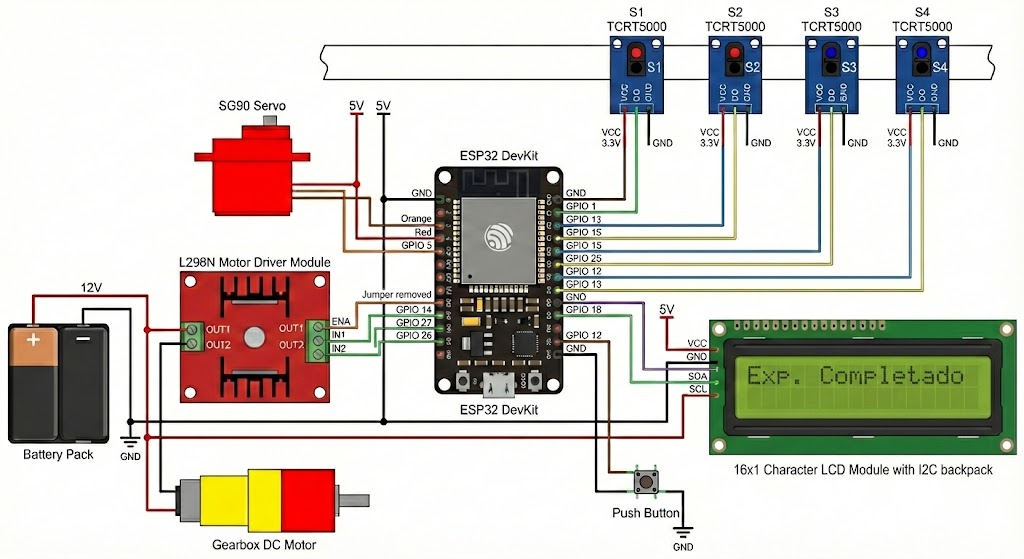
\includegraphics[width=\linewidth]{figures/Hardware connection diagram of the proposed prototype.png.jpg}
\caption{Esquem\'atico del m\'odulo de control~\cite{r50}.}
\label{fig:hardware_connection}
\end{figure}

\paragraph{Procesamiento Edge computing.}
Un aspecto central de la arquitectura propuesta es la implementaci\'on de procesamiento Edge computing en la Capa~1. El m\'odulo de control ejecuta localmente la detecci\'on de eventos mediante interrupciones de hardware y genera la marca temporal de cada evento \textbf{antes} de su transmisi\'on MQTT~\cite{r12}. Esto asegura que la latencia de la red WiFi---inherente a cualquier sistema distribuido---solo afecte la visualizaci\'on en la interfaz web, sin degradar la precisi\'on de las marcas temporales f\'isicas registradas. Este dise\~no sigue el modelo de Dizdarevic y Jukan~\cite{r7}, quienes destacan la reducci\'on efectiva de latencia mediante Edge computing en entornos educativos IoT, y es consistente con los principios de Hern\'andez \textit{et al.}~\cite{r51} para laboratorios remotos robustos ante desconexiones.

\subsection{Poblaci\'on, muestra y entorno experimental}

Este estudio no involucra una poblaci\'on de sujetos humanos, sino un sistema f\'isico instrumentado cuyo comportamiento se eval\'ua desde una perspectiva t\'ecnica. Se realizaron un total de 70 ensayos, correspondientes a 35 pruebas en modo presencial y 35 en modo remoto. El experimento se llev\'o a cabo en el laboratorio de f\'isica de la Pontificia Universidad Cat\'olica del Ecuador, sede Esmeraldas, que cuenta con un banco de trabajo nivelado, acceso a energ\'ia regulada y conectividad de red local a trav\'es de un punto de acceso WiFi. En este espacio se instalaron la pista tipo Hot Wheels\textsuperscript{\textregistered}~\cite{r18}, el carrito de baja fricci\'on~\cite{r19}, los cuatro sensores infrarrojos~\cite{r20}, el m\'odulo de control~\cite{r21,r53} y la c\'amara Insta360 Link~\cite{r36}. La Raspberry~Pi~4~\cite{r37} se ubic\'o en el mismo laboratorio y se conect\'o tanto al punto de acceso WiFi~\cite{r32} como a la red cableada institucional. La longitud efectiva de la pista es de 160~cm, a lo largo de la cual se distribuyeron los cuatro sensores de detecci\'on a intervalos de 53,2~cm.

\subsection{Procedimiento de implementaci\'on}

El procedimiento se organiz\'o en cuatro etapas. Primero, se realiz\'o un levantamiento de requisitos junto con el docente del curso de f\'isica. Se identificaron los eventos que el sistema deb\'ia registrar (paso del carrito por cada sensor), la informaci\'on m\'inima necesaria para describir el experimento y las condiciones aceptables de montaje. Con base en estos insumos, se defini\'o la arquitectura IoT, especificando componentes de hardware, servicios de software y el flujo de datos entre el ESP32, el servidor MQTT, el backend y la aplicaci\'on web.

En una segunda fase, se construy\'o el montaje f\'isico de la pista y se instalaron los sensores infrarrojos en posiciones fijas a lo largo del recorrido del carrito. El m\'odulo de control fue programado mediante el Arduino IDE para leer los estados de los sensores y enviar mensajes MQTT con marcas temporales al servidor desplegado en la Raspberry Pi. Durante esta fase se realizaron pruebas unitarias para verificar la lectura correcta de sensores, la conectividad WiFi y la publicaci\'on en los t\'opicos MQTT definidos.

A continuaci\'on, se configur\'o el entorno experimental y se ejecutaron los ensayos. El punto de partida del carrito, la inclinaci\'on de la pista y las posiciones de los sensores se fijaron, manteniendo estos par\'ametros constantes en todas las pruebas. Las series de ensayos se realizaron en dos modalidades: operaci\'on remota a trav\'es de la interfaz web, en la cual el usuario activaba el experimento y los tiempos de detecci\'on se registraban autom\'aticamente; y operaci\'on presencial utilizando un montaje de referencia sin el componente IoT, que sirvi\'o como l\'inea base para la comparaci\'on.

Finalmente, se realiz\'o la validaci\'on t\'ecnica. Los datos generados por ambos sistemas se recopilaron y organizaron en tablas comparativas por sensor y por repetici\'on. Se evalu\'o la coincidencia de los tiempos de detecci\'on entre ambas modalidades y se documentaron cualitativamente los incidentes relacionados con la estabilidad.

\begin{figure}[H]
\centering
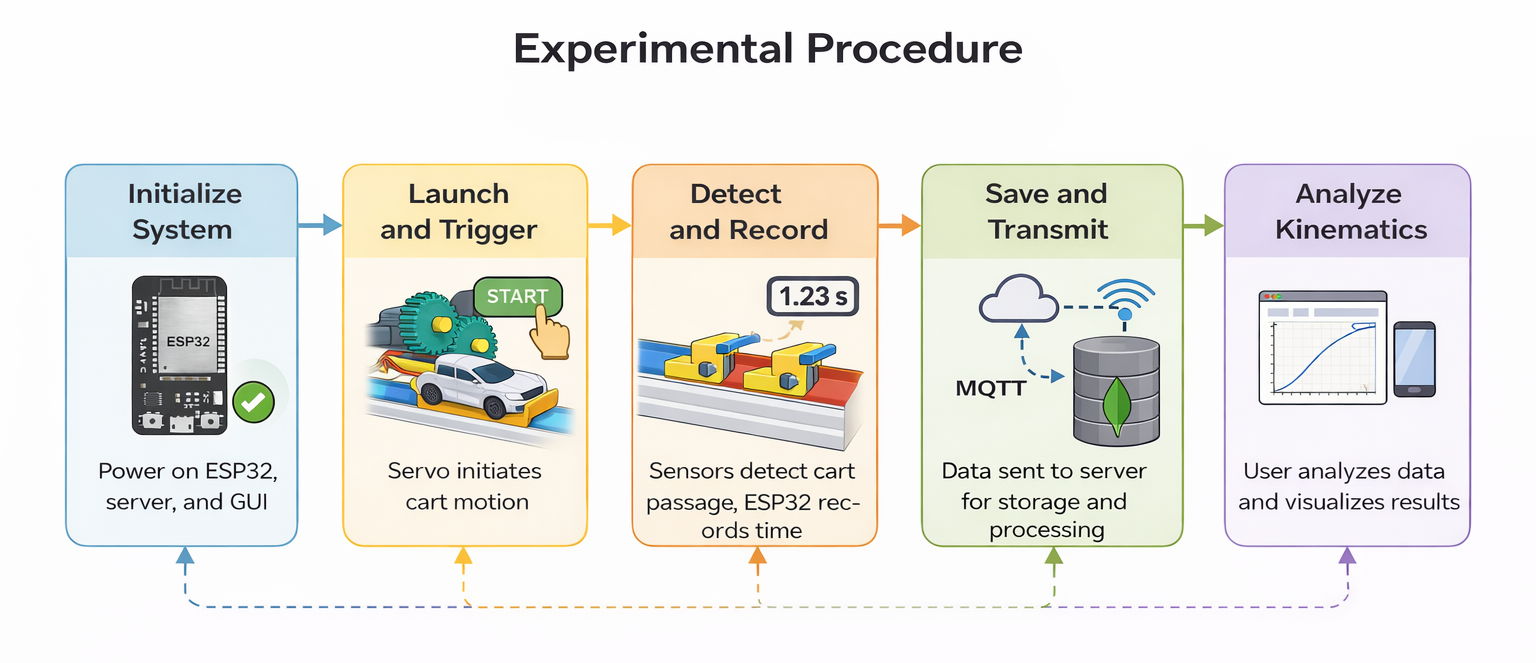
\includegraphics[width=\linewidth]{figures/Experimental procedure flowchart.png}
\caption{Flujo de datos durante la operaci\'on del laboratorio~\cite{r49}.}
\label{fig:flujo-datos}
\end{figure}

\subsection{M\'etricas de evaluaci\'on}

En la validaci\'on t\'ecnica, el an\'alisis se centra en cuantificar el grado de asociaci\'on y concordancia entre las mediciones obtenidas en la modalidad presencial y las registradas por el sistema IoT. Como m\'etrica fundamental de desempe\~no se adopta el coeficiente de correlaci\'on de Pearson ($r$), calculado independientemente para cada sensor (S1 a S4). Dado que los ensayos en ambas modalidades fueron ejecutados como eventos f\'isicos independientes y no emparejados, el an\'alisis no busca correspondencia punto a punto, sino que certifica que ambos sistemas capturan la din\'amica del MRUA de manera consistente.

\begin{equation}
r = \\frac{\\sum_{i=1}^{n} (x_i - \\bar{x})(y_i - \\bar{y})}{\\sqrt{\\sum_{i=1}^{n} (x_i - \\bar{x})^2} \\sqrt{\\sum_{i=1}^{n} (y_i - \\bar{y})^2}}
\label{eq:pearson}
\end{equation}

Donde $x_i$ representa los tiempos medidos en la modalidad presencial e $y_i$ los tiempos medidos en la modalidad remota para $n=35$ ensayos por modalidad. El an\'alisis se complementa con el m\'etodo de Bland--Altman~\cite{bland1986}, que eval\'ua directamente los l\'imites de concordancia entre ambas modalidades~\cite{giavarina2015}.

%========================================================
\section{Resultados y discusi\'on}

\subsection{Fundamento te\'orico}

La aceleraci\'on te\'orica esperada es:
\begin{equation}
  a_{\text{te\'orica}} = g \cdot \sin\theta
  \label{eq:mruateorico}
\end{equation}
donde $g = 9{,}81$~m/s$^2$. La velocidad media en cada segmento es:
\begin{equation}
  \bar{v}_{i,i+1} = \frac{\Delta d}{t_{i+1} - t_i}
  \label{eq:velocidad}
\end{equation}
La aceleraci\'on media se estima mediante:
\begin{equation}
  a_{\text{exp}} = \frac{\Delta \bar{v}}{\Delta t}
  \label{eq:aceleracion}
\end{equation}

\subsection{Montaje experimental}

La Figura~\ref{fig:montaje_detalles} presenta la implementaci\'on f\'isica del prototipo integrado con la capa de sensado.

\begin{figure}[H]
\centering
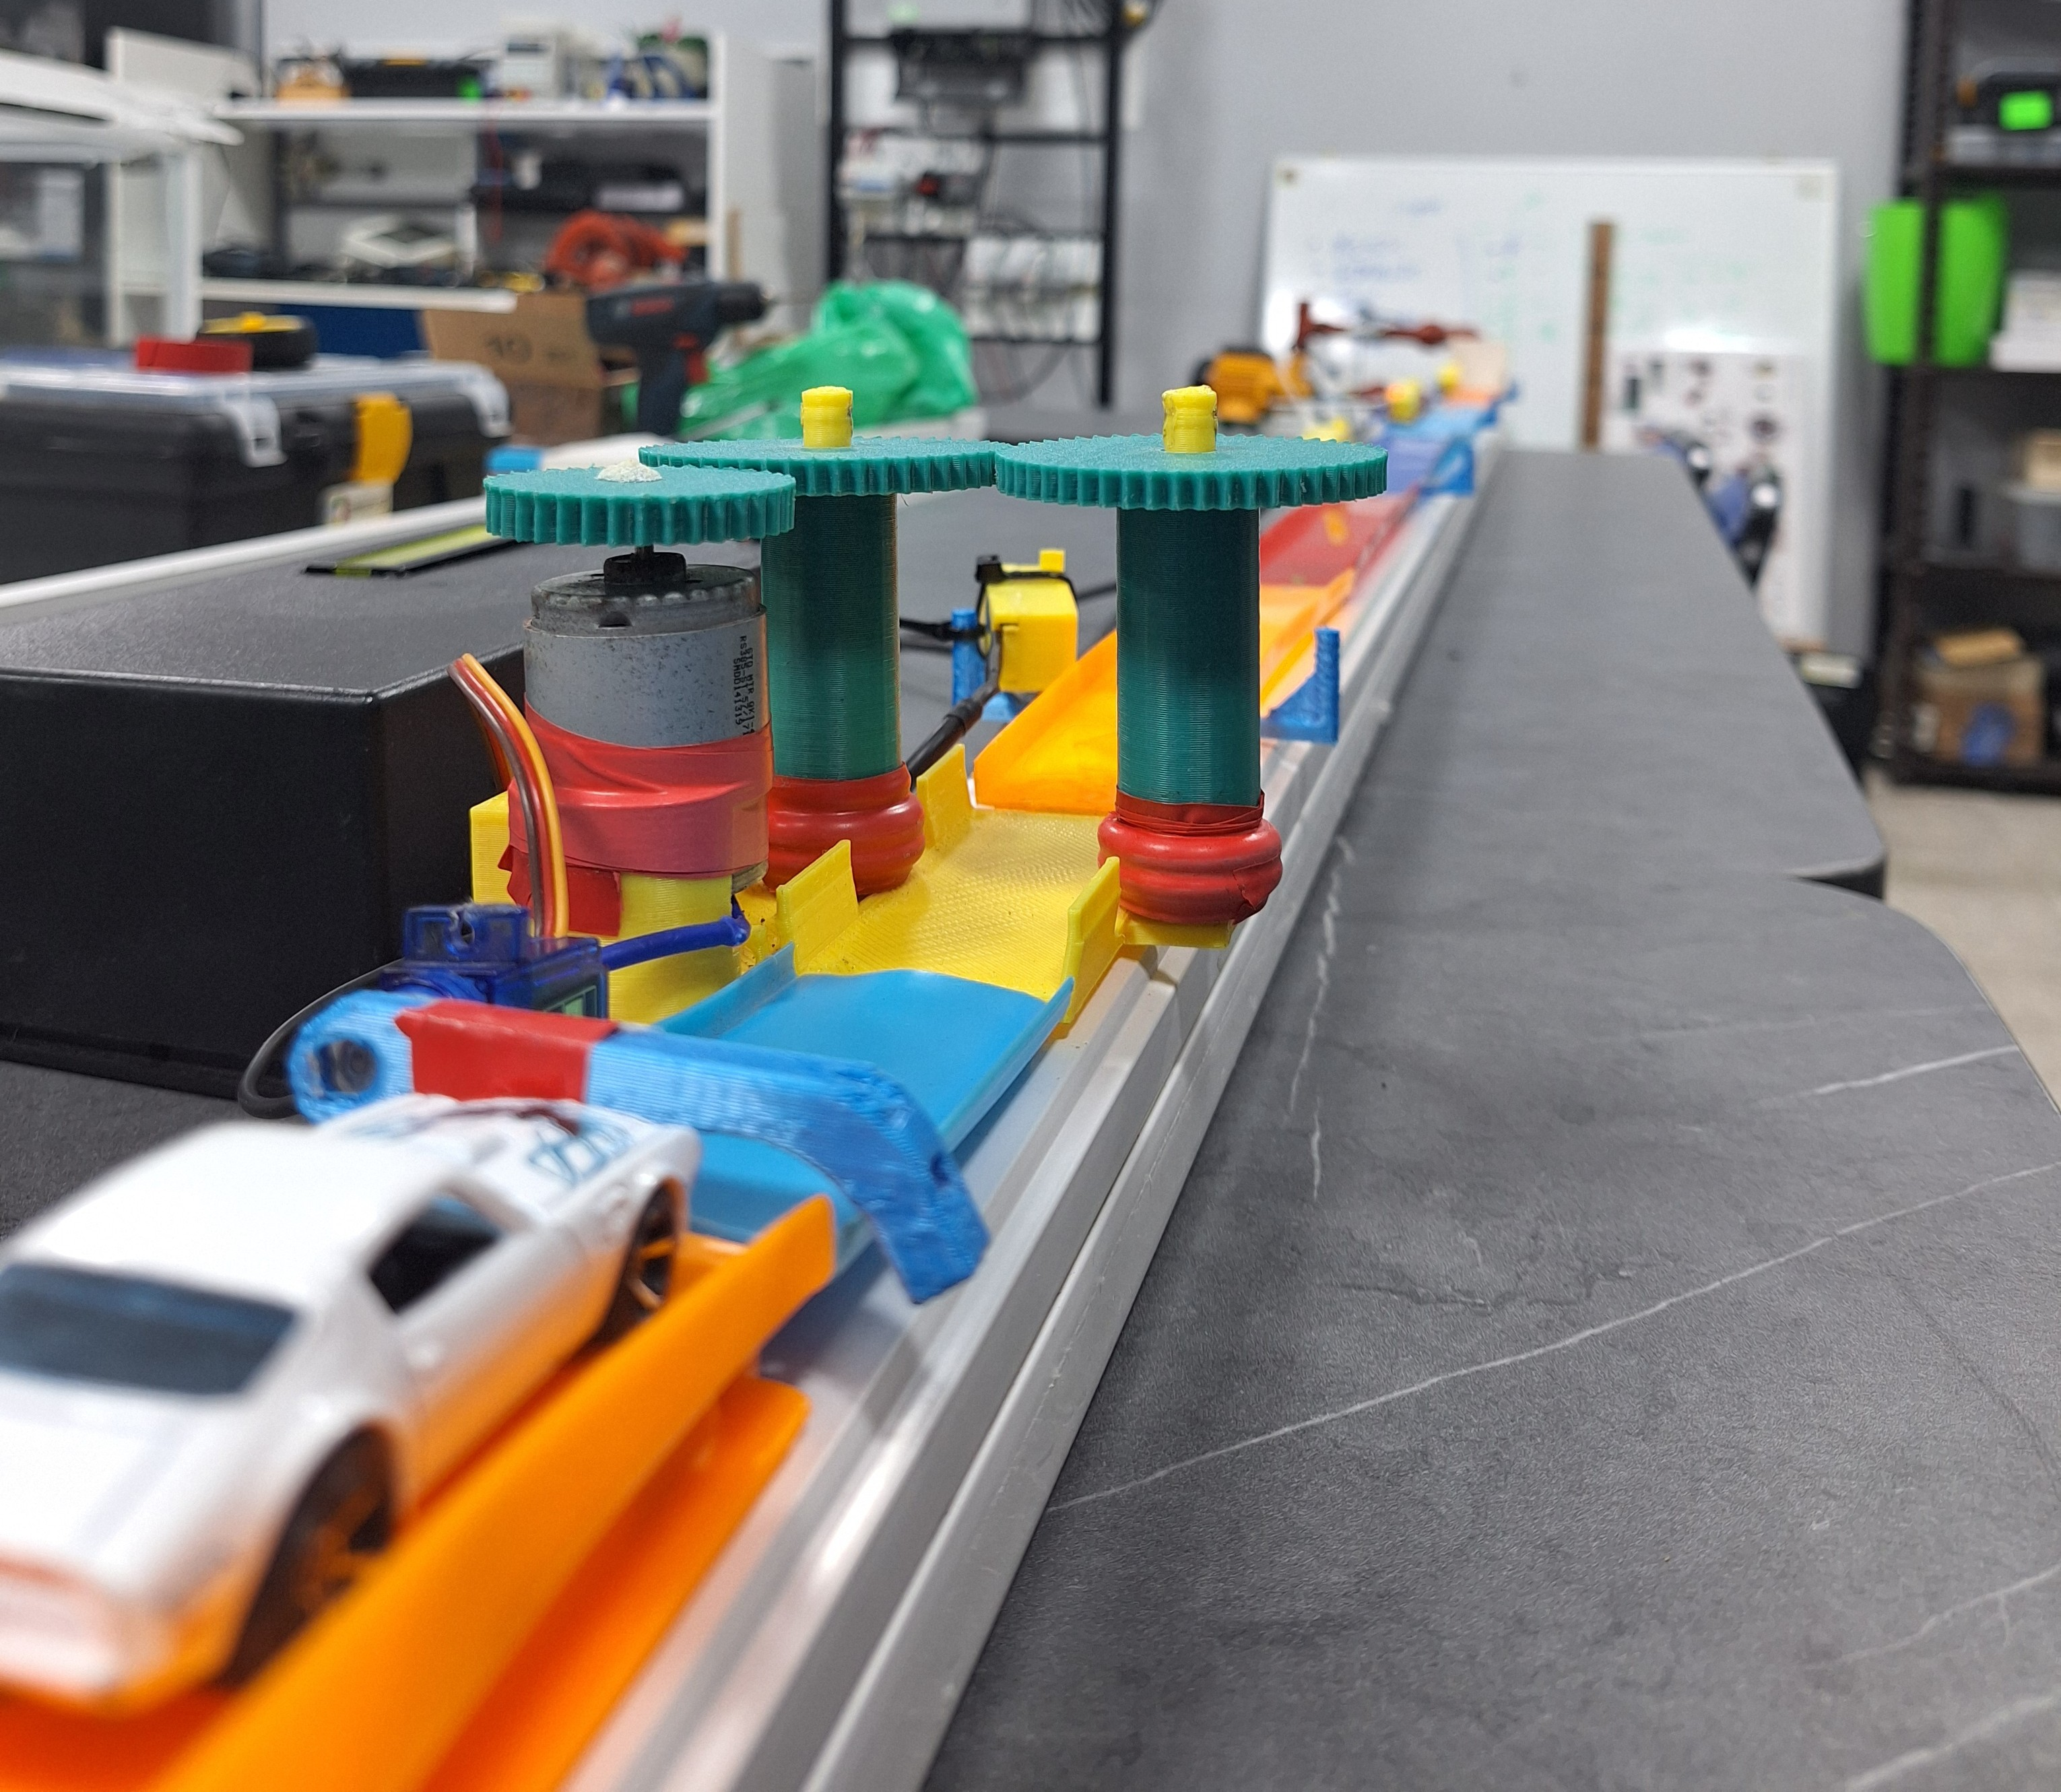
\includegraphics[width=\linewidth]{figures/setup_overview_completo.jpg}
\caption{Vista general del montaje experimental de MRUA basado en IoT.}
\label{fig:montaje_detalles}
\end{figure}

Se desarroll\'o una interfaz de usuario web para la interacci\'on remota (Figura~\ref{fig:interfaz_web}).

\begin{figure}[H]
\centering
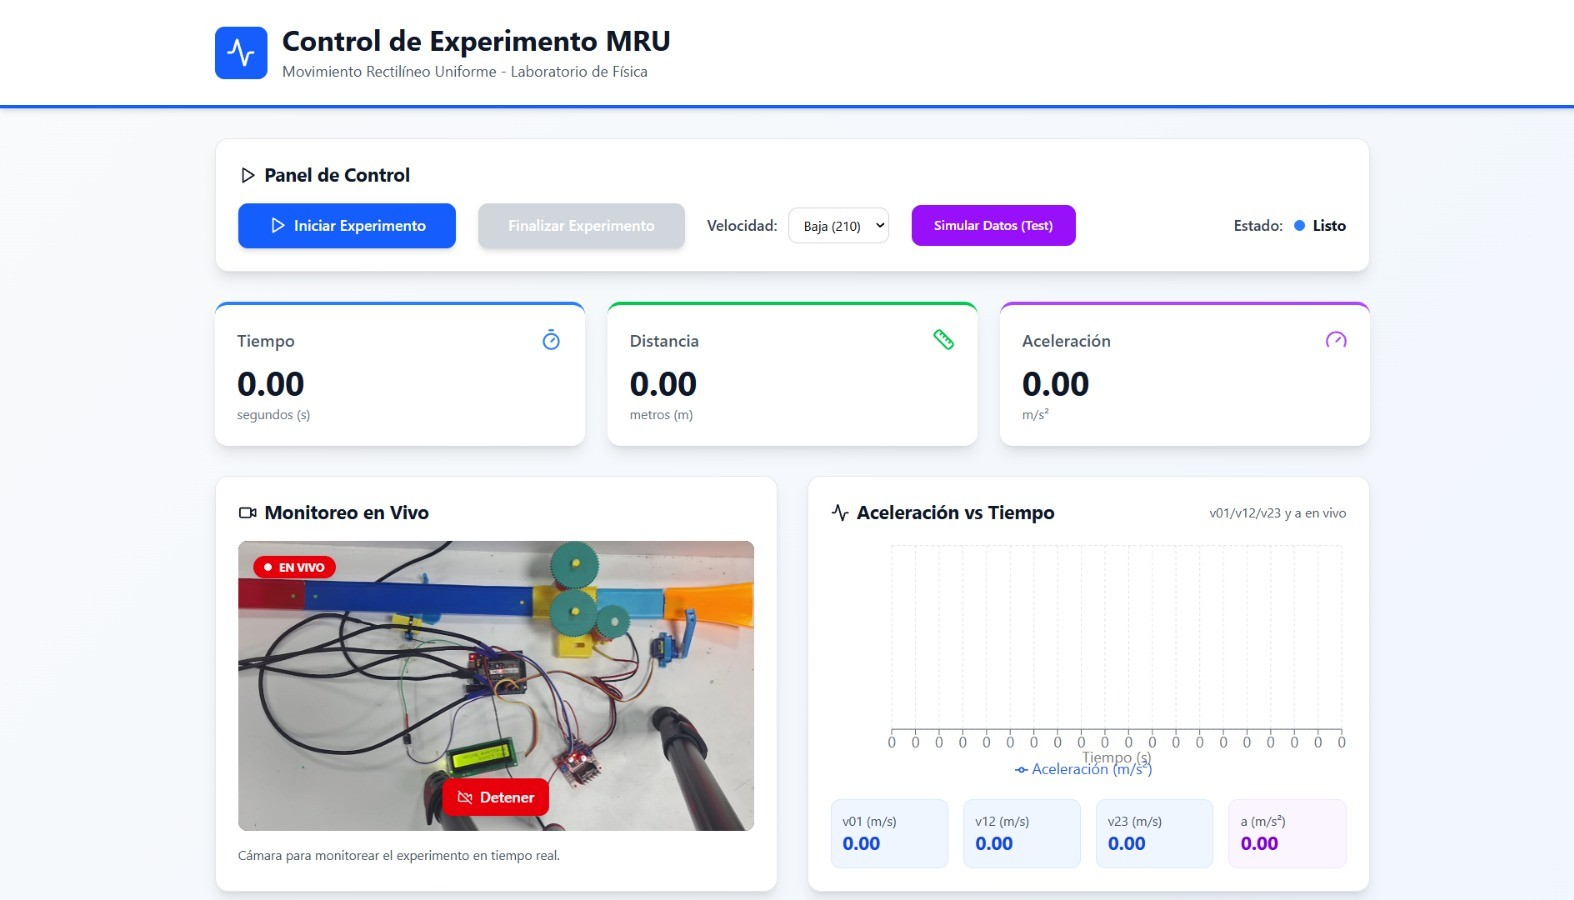
\includegraphics[width=\linewidth]{figures/InterfazWeb.jpg}
\caption{Interfaz web para el control y monitoreo remoto del experimento.}
\label{fig:interfaz_web}
\end{figure}

\subsection{Resumen estad\'istico global}

La Tabla~\ref{tab:resumen_global} sintetiza los resultados estad\'isticos por sensor. Las diferencias medias entre modalidades son inferiores a 0,01~s en todos los puntos de medici\'on con $\Delta\sigma < 0{,}02$~s.

\begin{table}[H]
\caption{Resumen estad\'istico comparativo por sensor ($n = 35$ por modalidad).}
\label{tab:resumen_global}
\centering
\scriptsize
\begin{tabular}{lrrrrr}
\toprule
\textbf{Sensor} & $\bar{x}_P$ & $\bar{y}_R$ & $\sigma_P$ & $\sigma_R$ & $r$ \\
\midrule
S1 (ref.) & 0,000 & 0,000 & 0,000 & 0,000 & {---} \\
S2        & 1,09  & 1,09  & 0,15  & 0,16  & {---} \\
S3        & 1,54  & 1,54  & 0,22  & 0,22  & {---} \\
S4        & 1,89  & 1,89  & 0,27  & 0,27  & {---} \\
\bottomrule
\end{tabular}
\end{table}

\subsection{An\'alisis de concordancia Bland--Altman}

Se aplic\'o el m\'etodo de Bland--Altman~\cite{bland1986}. Los resultados se presentan en la Tabla~\ref{tab:bland_altman}. El sesgo medio ($\overline{d}$) es pr\'acticamente nulo en todos los sensores ($|\overline{d}| < 0{,}002$~s), demostrando la ausencia de error sistem\'atico. La amplitud de los l\'imites de concordancia ($\pm$0,46--0,80~s) refleja la variabilidad f\'isica de los ensayos no emparejados, no limitaciones instrumentales.

\begin{table}[H]
\caption{An\'alisis Bland--Altman por sensor.}
\label{tab:bland_altman}
\centering
\scriptsize
\begin{tabular}{lcccc}
\toprule
\textbf{Sensor} &
$\overline{d}$ (s) &
$\sigma_d$ (s) &
\textbf{Inferior} &
\textbf{Superior} \\
\midrule
S2 & 0,000 & 0,234 & $-$0,459 & 0,460 \\
S3 & 0,002 & 0,332 & $-$0,649 & 0,653 \\
S4 & 0,001 & 0,408 & $-$0,799 & 0,800 \\
\bottomrule
\end{tabular}
\end{table}

\begin{figure}[H]
    \centering
    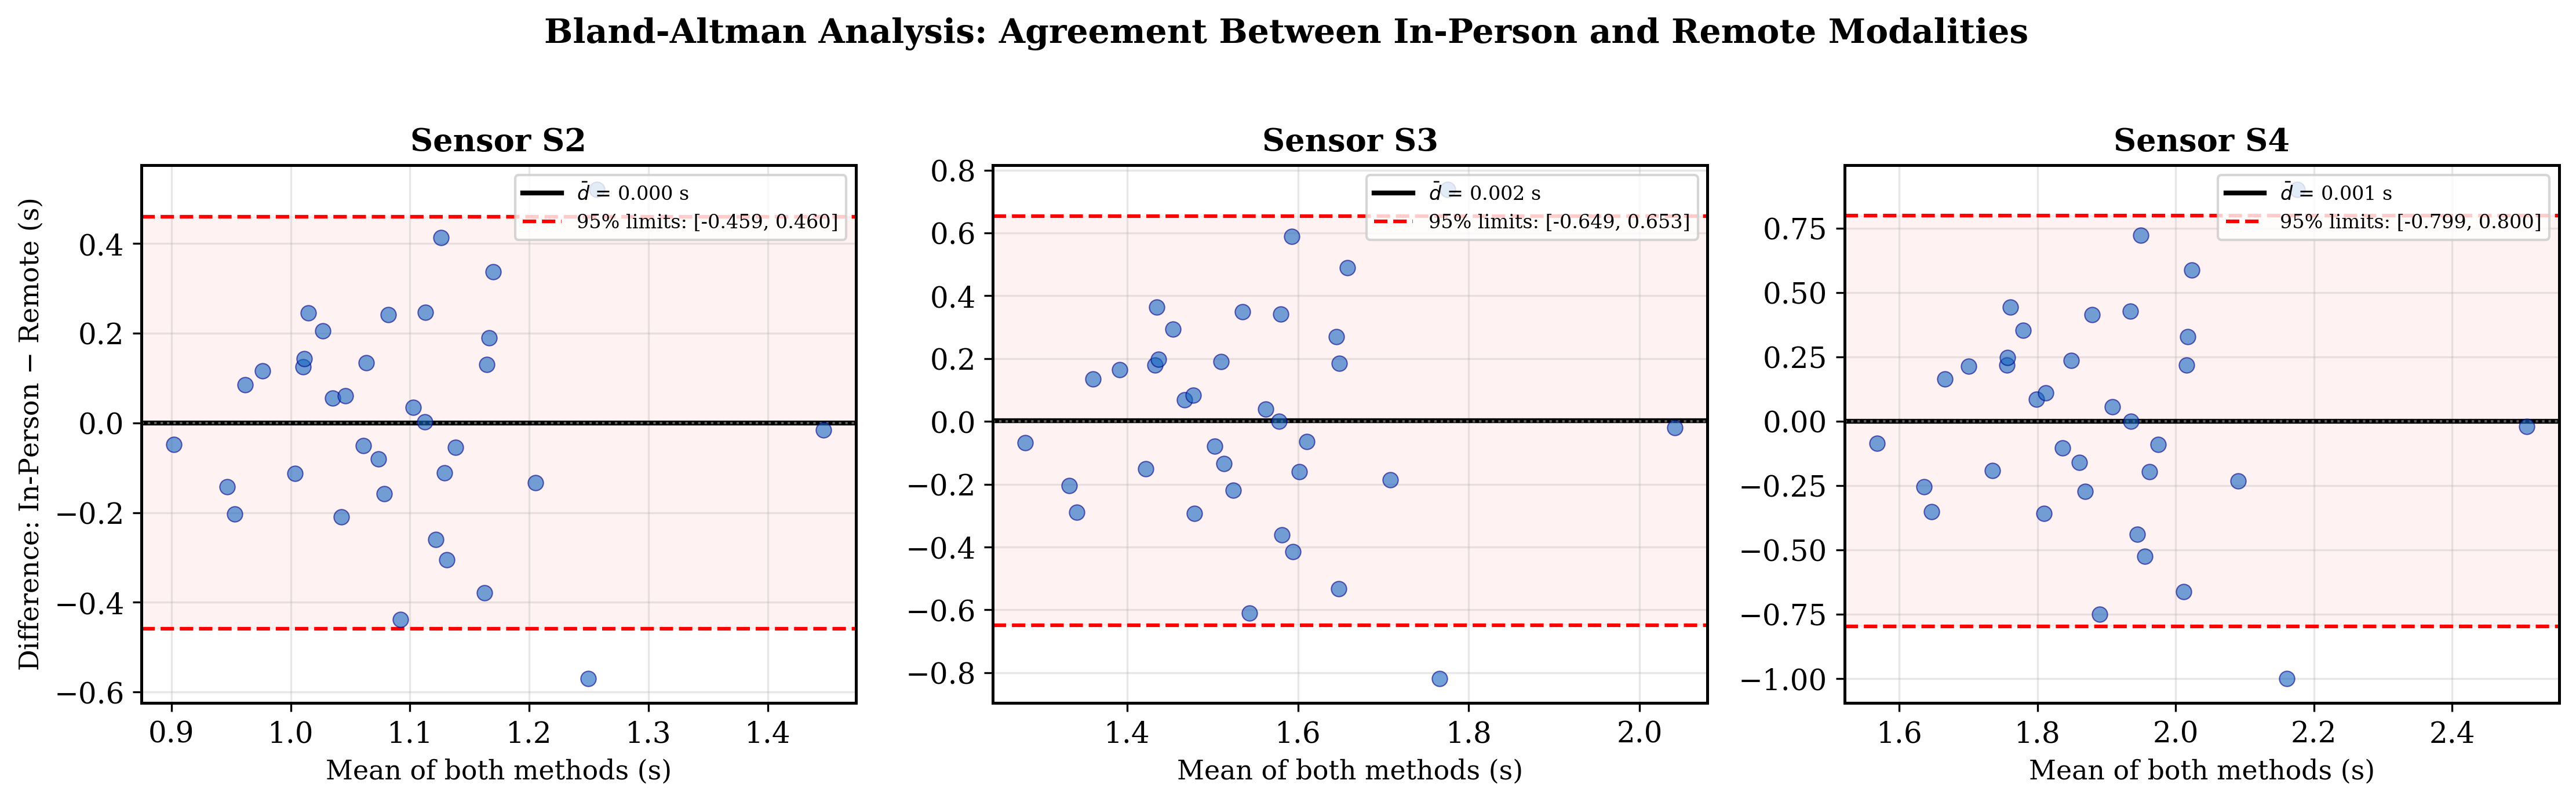
\includegraphics[width=\linewidth]{figures/bland_altman_english_white.png}
    \caption{An\'alisis Bland--Altman para los sensores S2, S3 y S4. La l\'inea negra continua representa el sesgo medio; las l\'ineas rojas punteadas delimitan los l\'imites de concordancia al 95\%.}
    \label{fig:bland_altman}
\end{figure}

\subsection{An\'alisis cinem\'atico global}

La Figura~\ref{fig:vel_profile} muestra el perfil de velocidad media para ambas modalidades utilizando la Ecuaci\'on~\ref{eq:velocidad}. Las curvas son pr\'acticamente indistinguibles.

\begin{figure}[H]
  \centering
  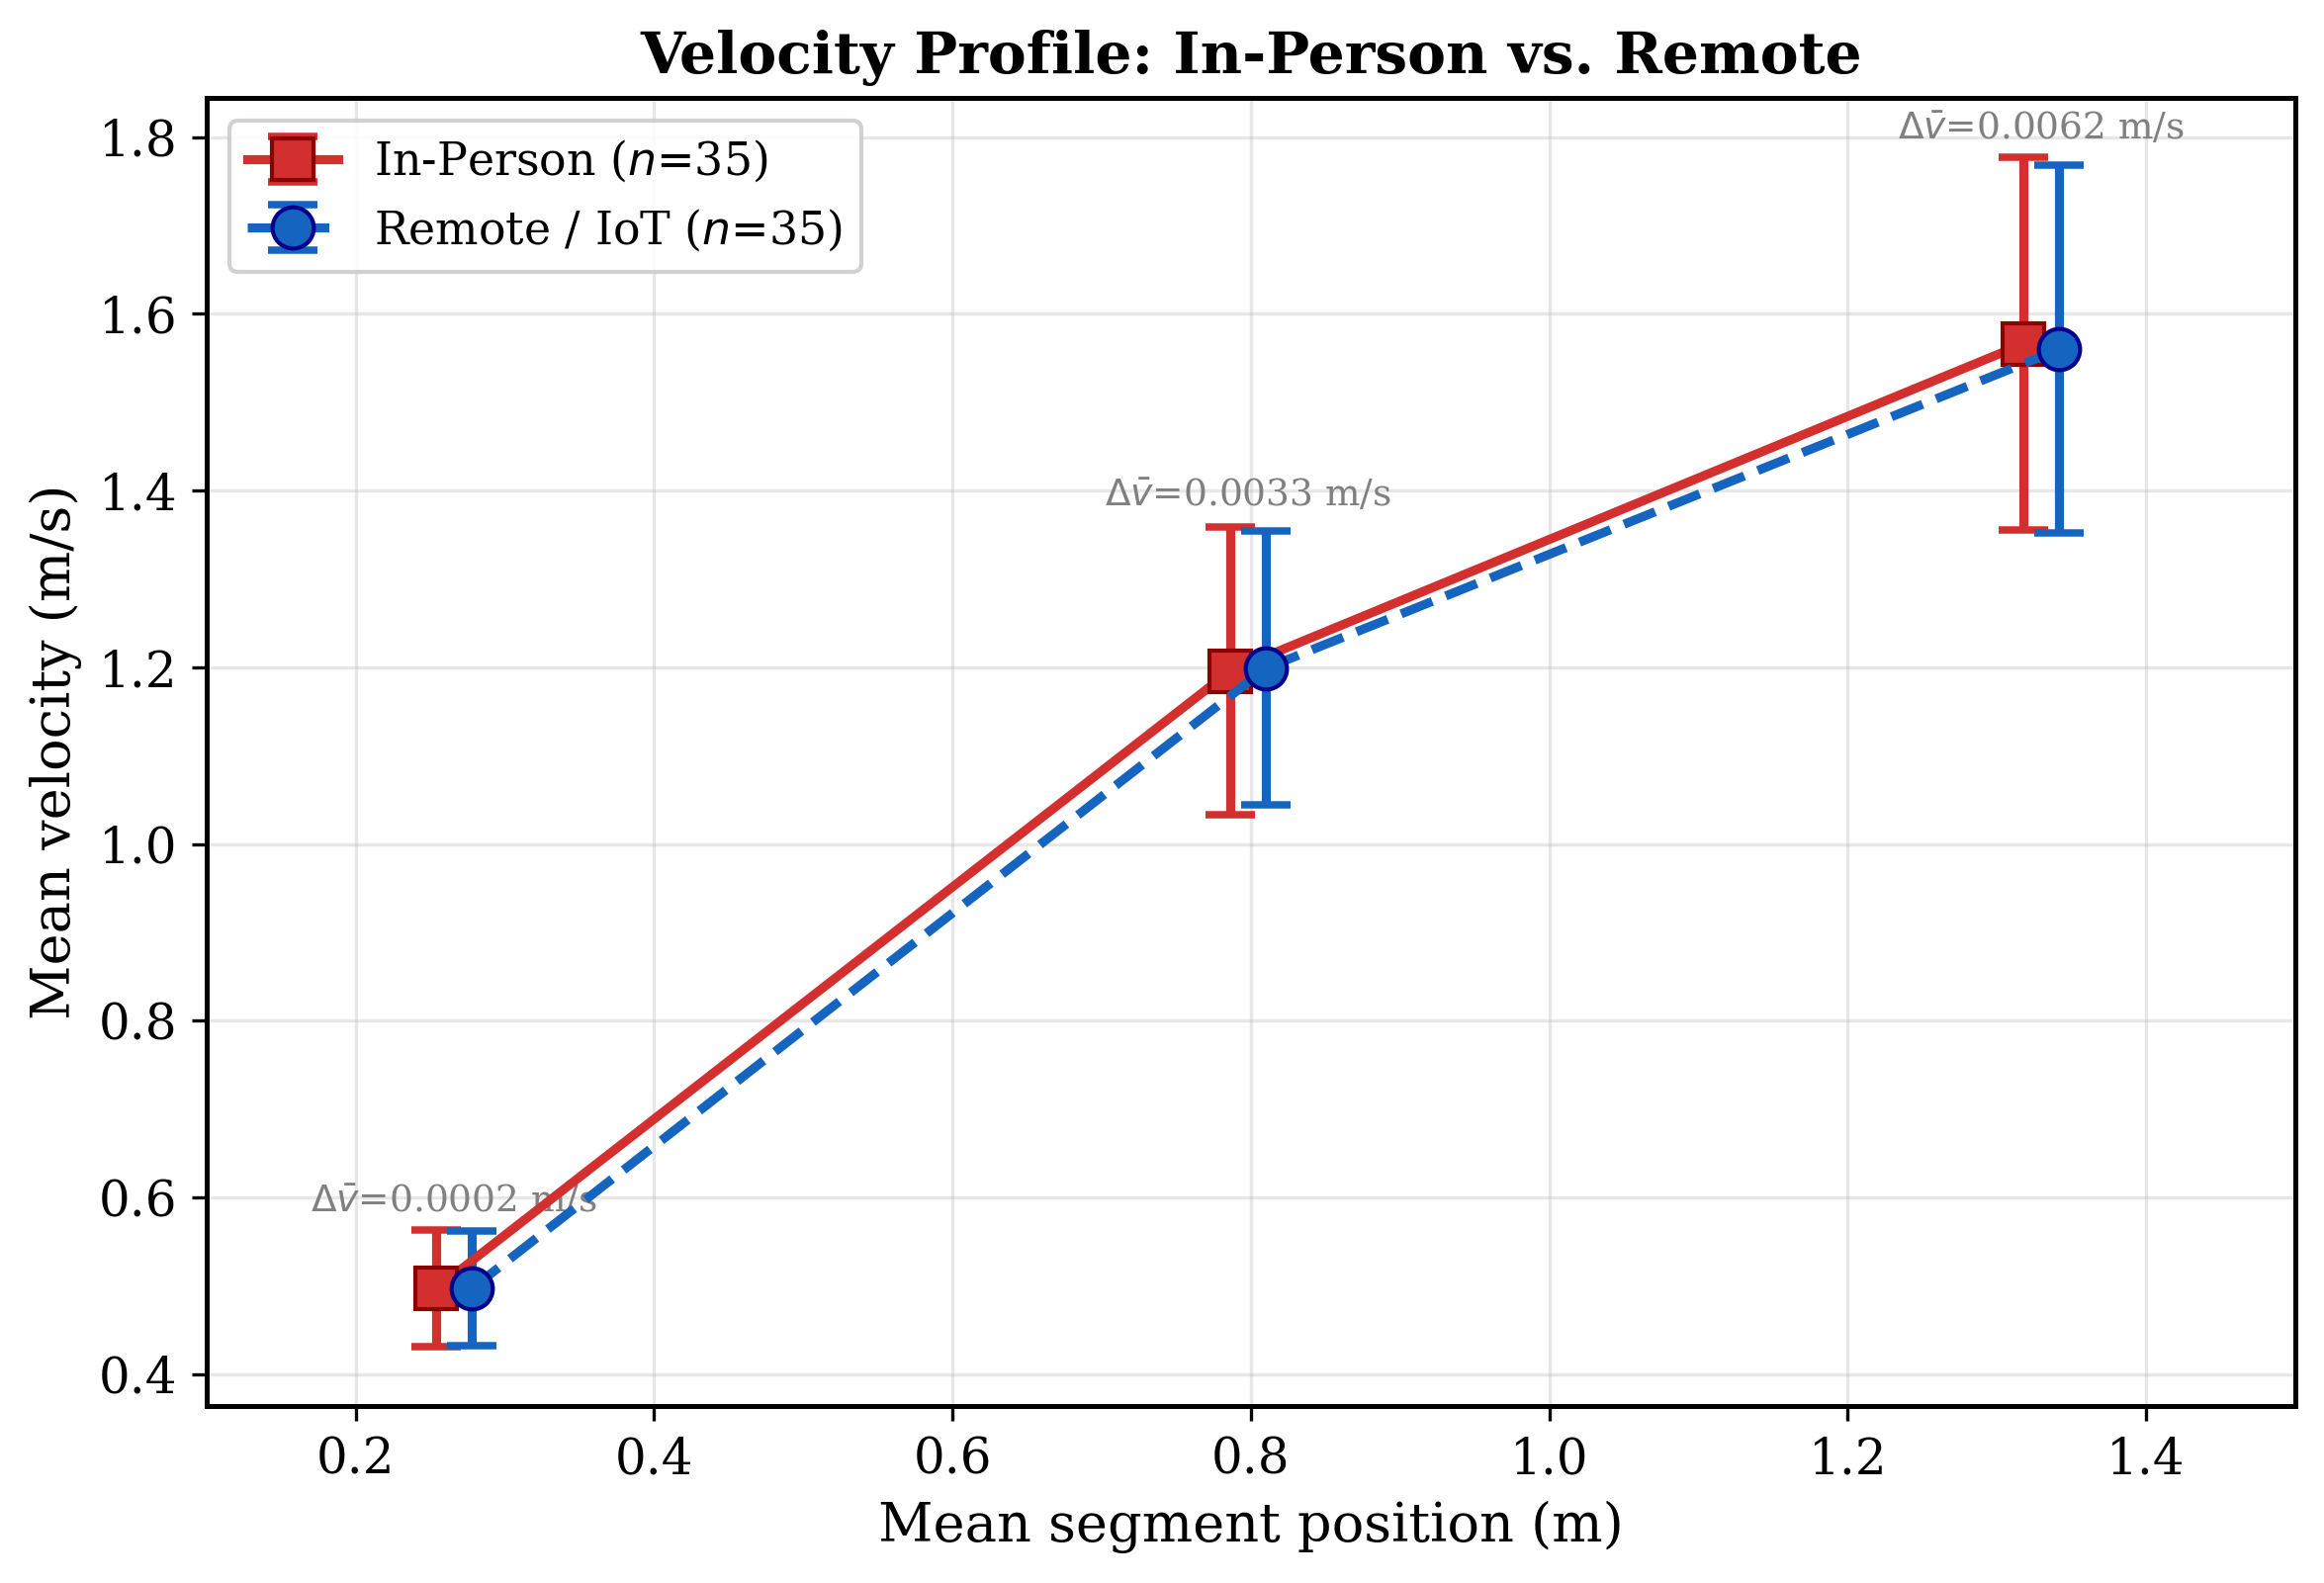
\includegraphics[width=\linewidth]{figures/velocity_profile.png}
  \caption{Perfil de velocidad media vs. posici\'on del segmento para las modalidades remota (azul) y presencial (rojo). Las barras de error representan $\pm 1\sigma$.}
  \label{fig:vel_profile}
\end{figure}

La Figura~\ref{fig:accel_box} presenta la distribuci\'on de la aceleraci\'on experimental. Ambas modalidades exhiben medias id\'enticas ($\mu \approx 0{,}95$~m/s$^2$) con desviaciones est\'andar similares.

\begin{figure}[H]
  \centering
  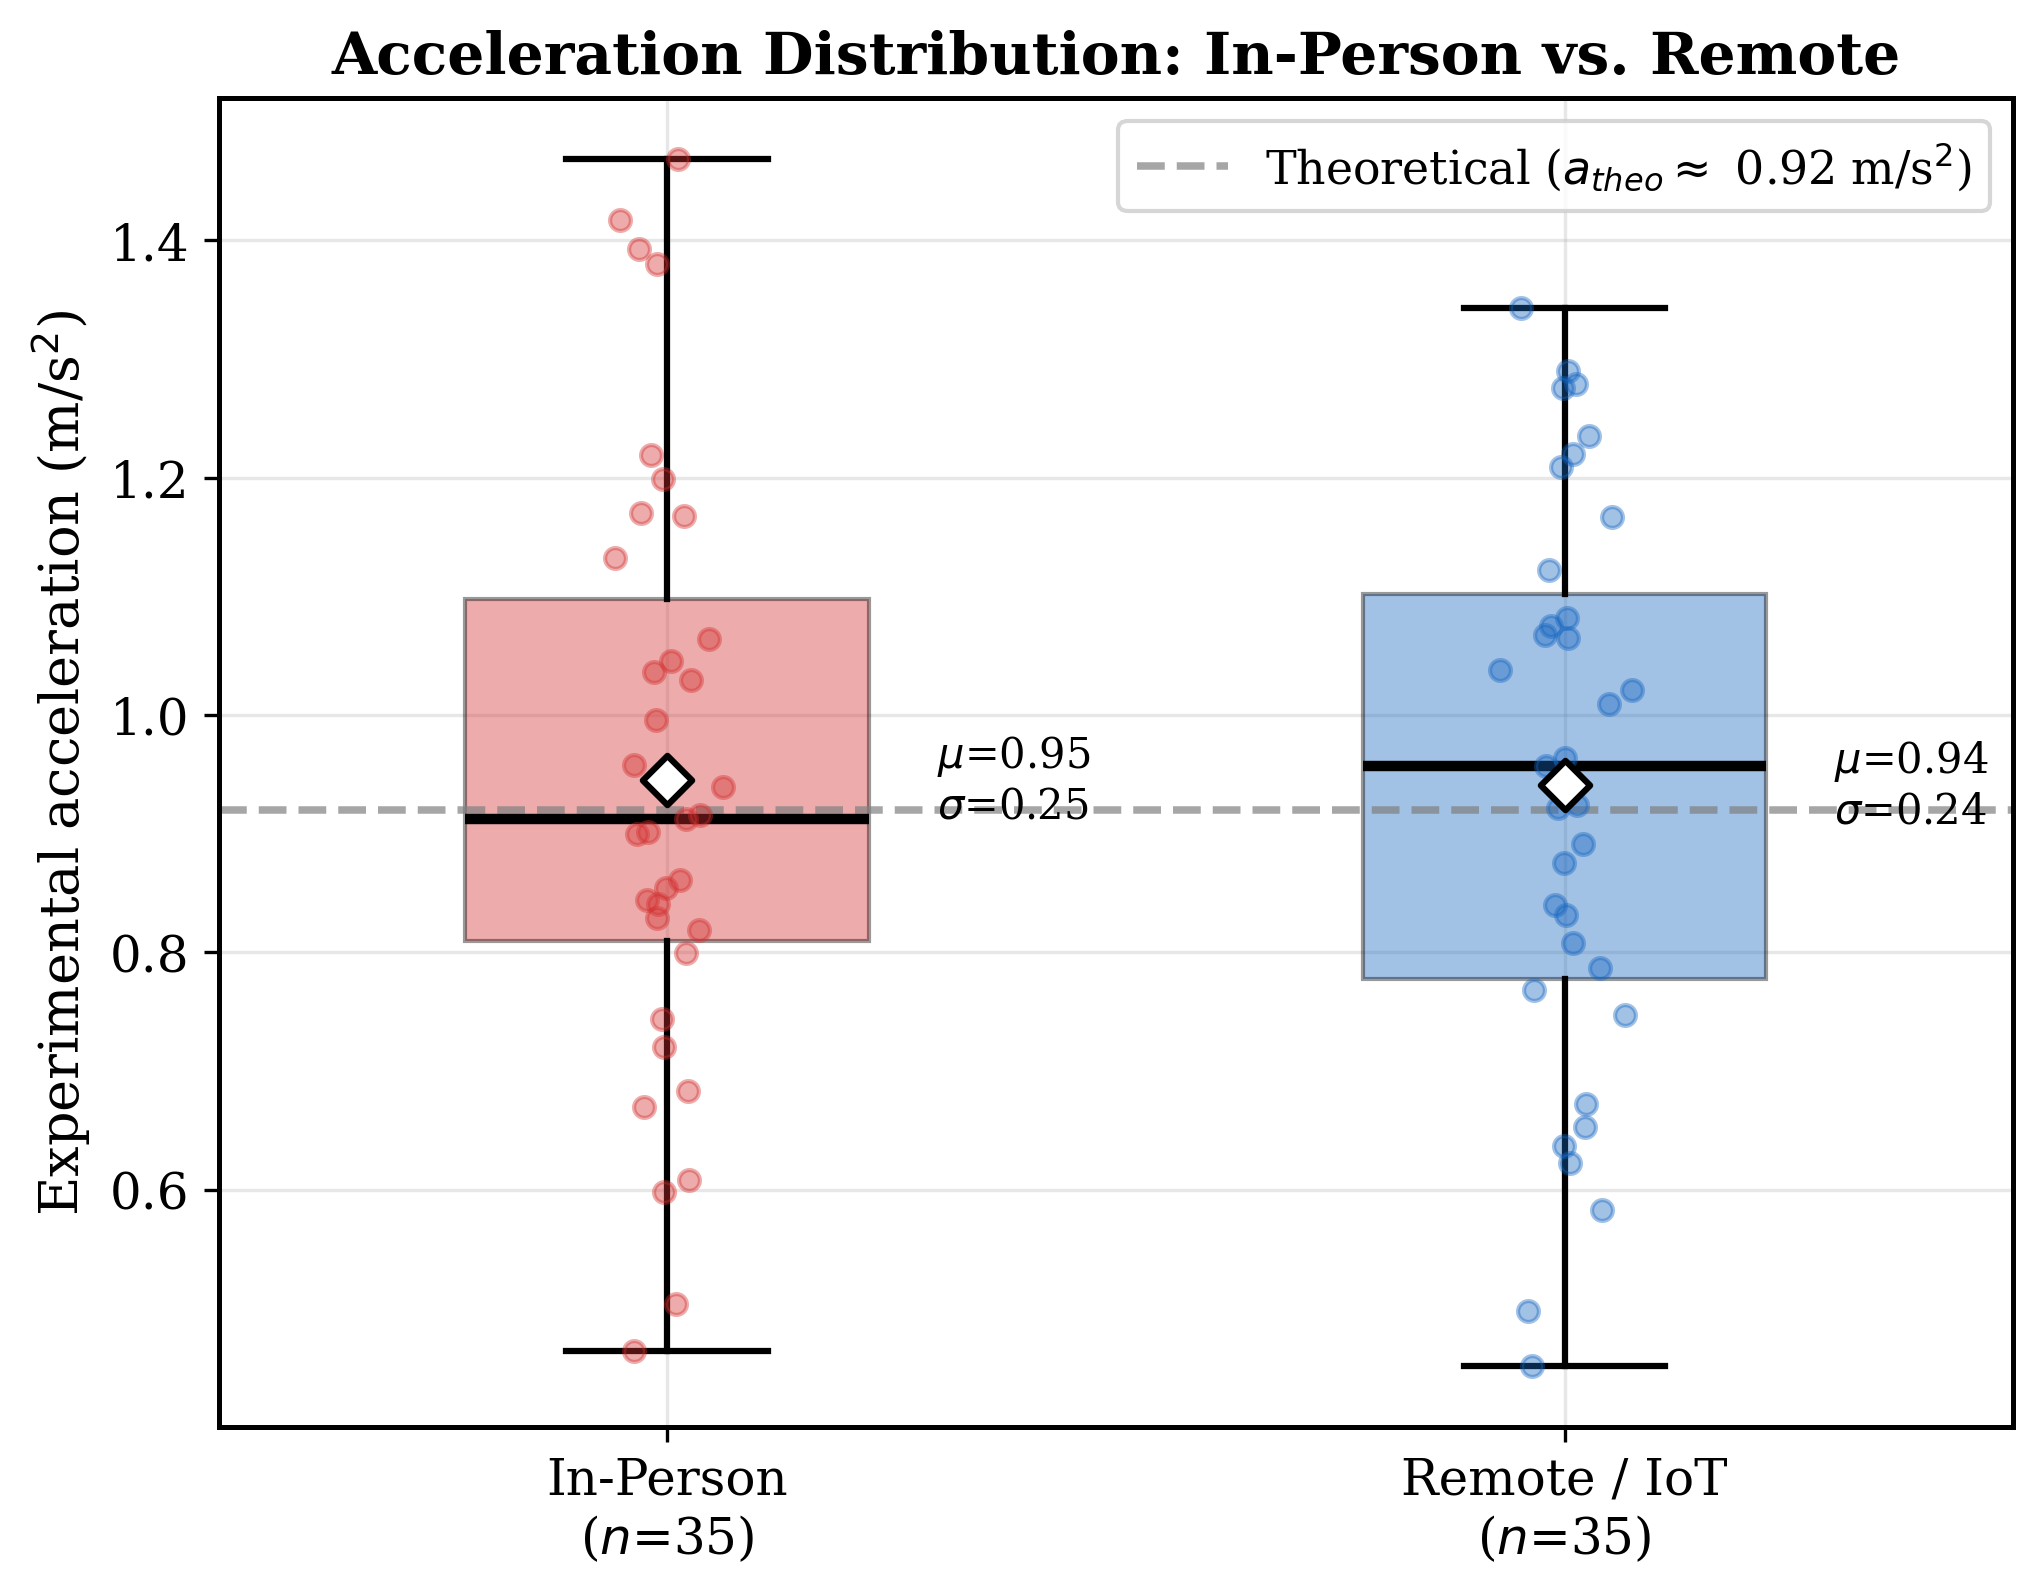
\includegraphics[width=\linewidth]{figures/acceleration_boxplot.png}
  \caption{Distribuci\'on de la aceleraci\'on experimental estimada para las modalidades remota y presencial ($n = 35$ cada una).}
  \label{fig:accel_box}
\end{figure}

La Figura~\ref{fig:mrua_teorico} compara los datos experimentales con el modelo te\'orico de MRUA. La diferencia del 3,3\% entre los valores experimental ($\mu \approx 0{,}95$~m/s$^2$) y te\'orico ($a \approx 0{,}92$~m/s$^2$) se encuentra dentro del margen esperado~\cite{r10}.

\begin{figure}[H]
  \centering
  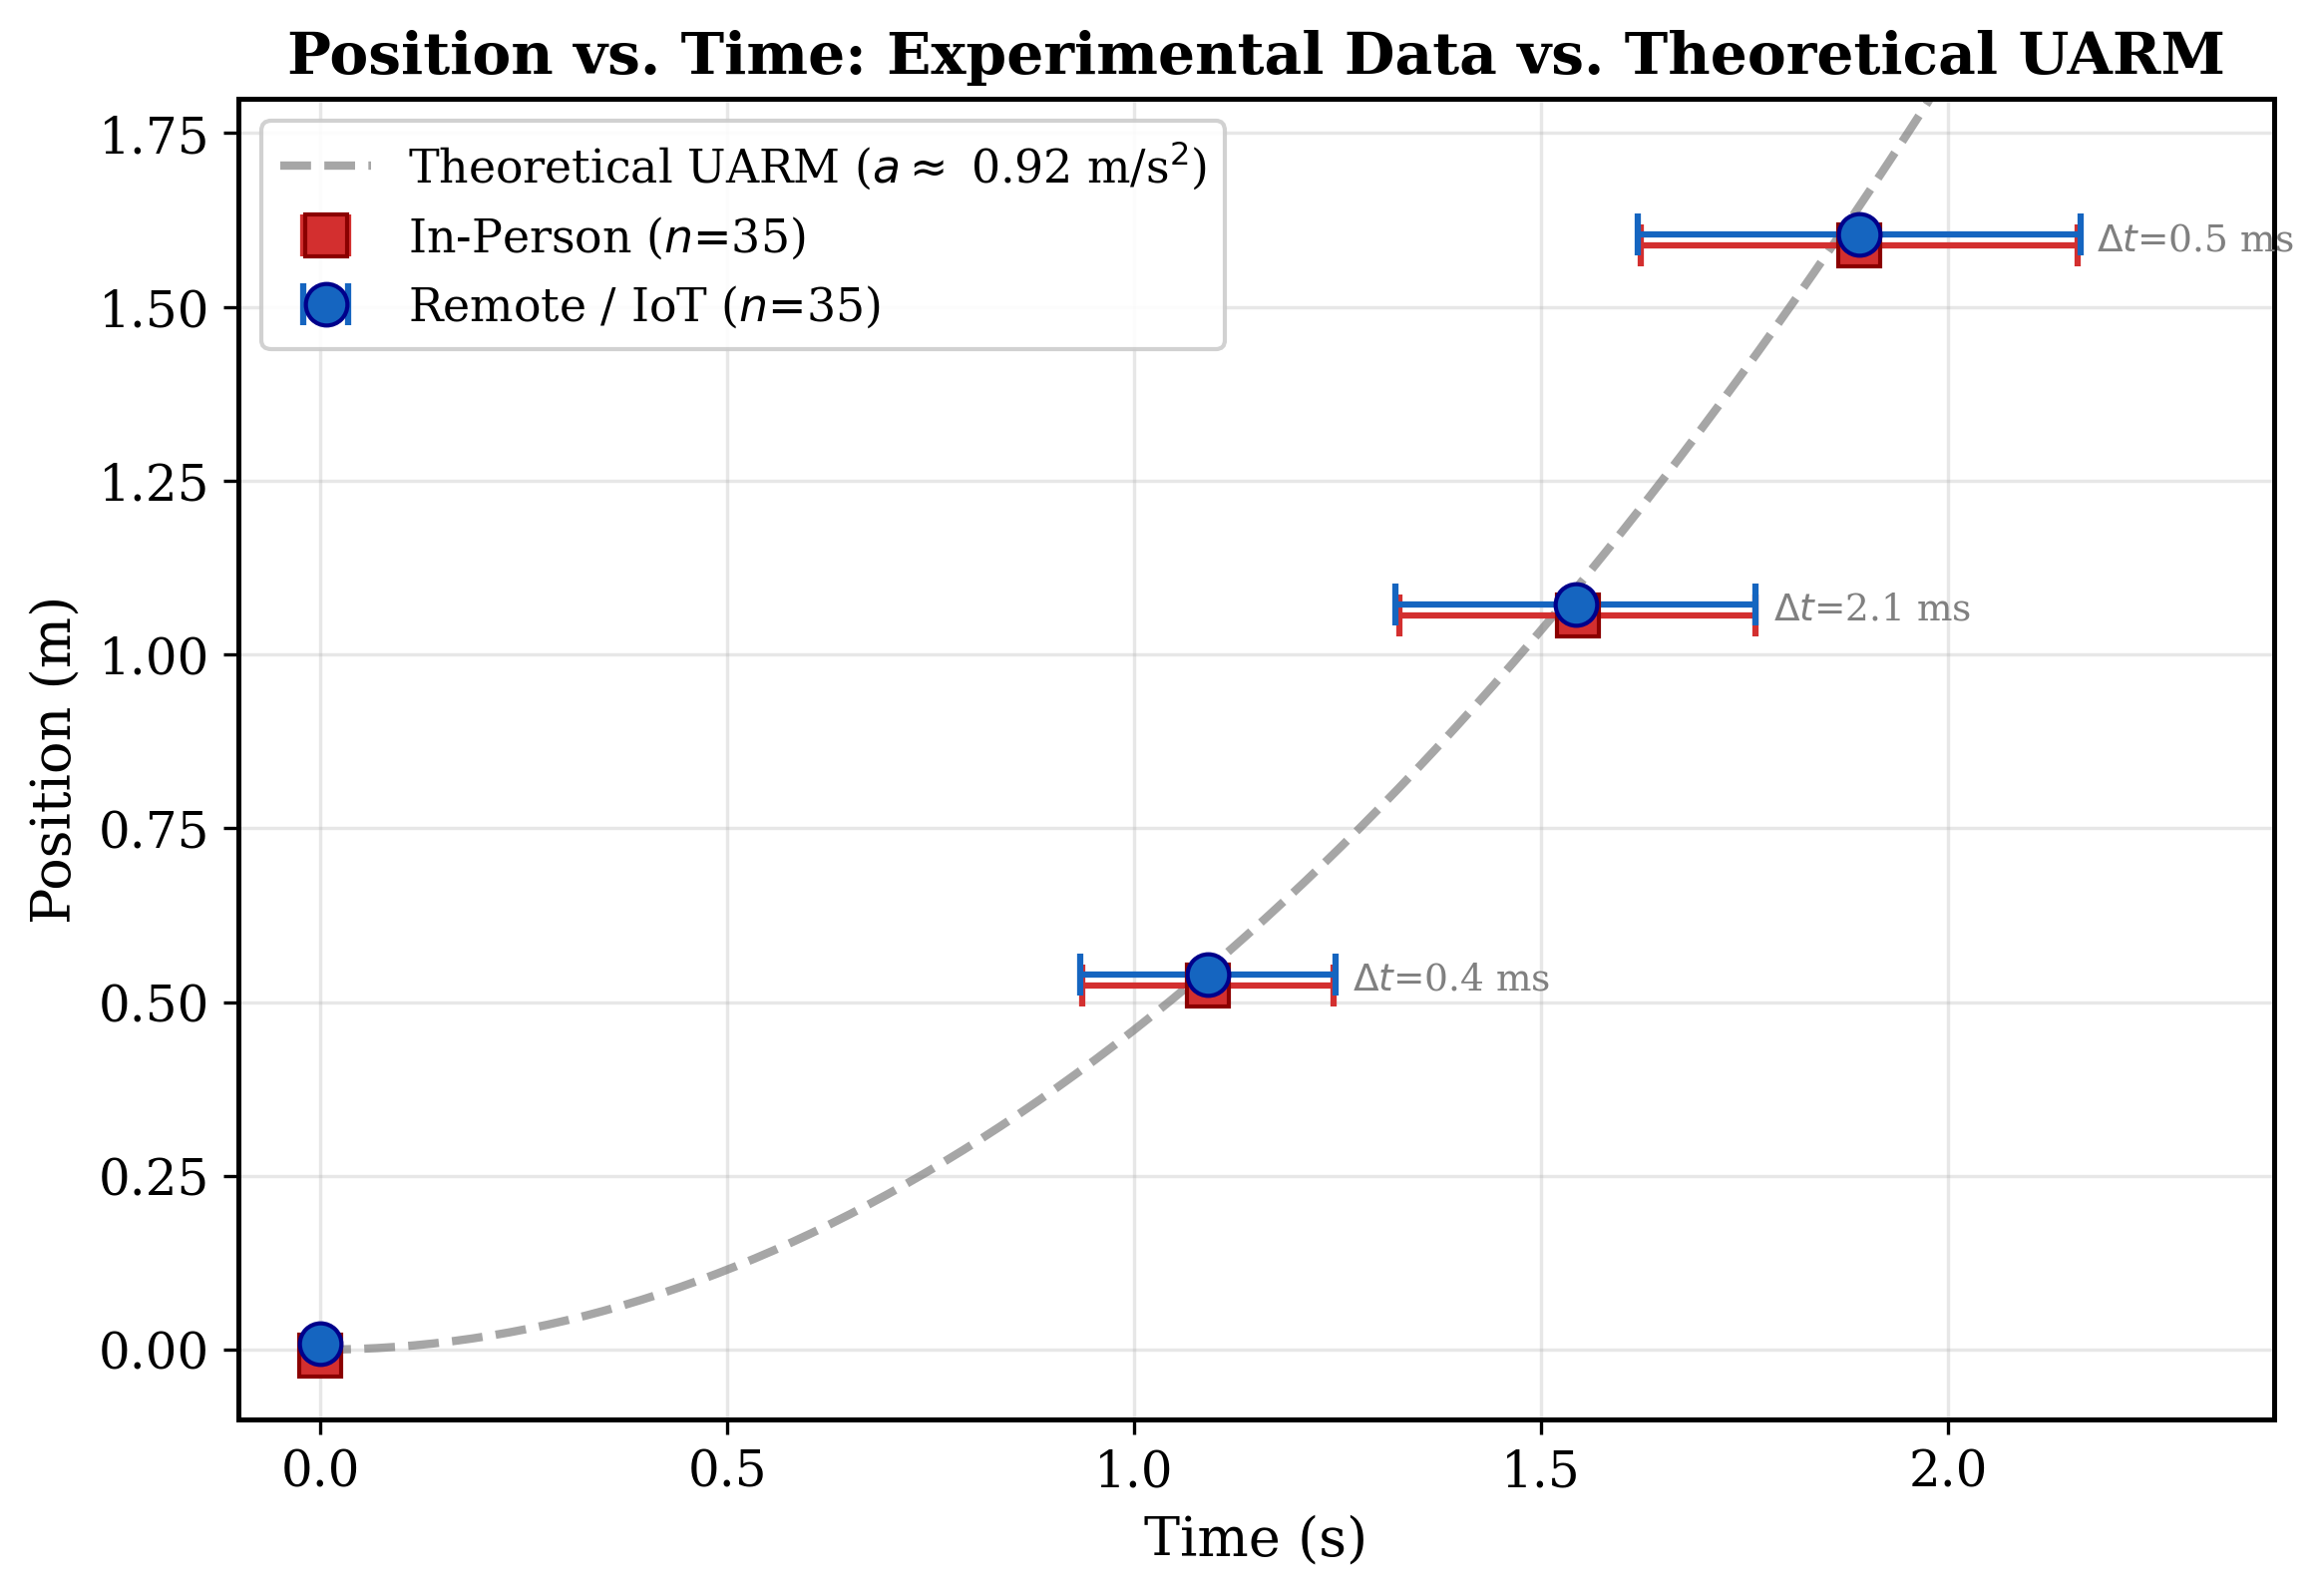
\includegraphics[width=\linewidth]{figures/experimental_vs_theoretical_mrua.png}
  \caption{Posici\'on vs. tiempo: modelo te\'orico de MRUA (gris punteado) y datos experimentales de las modalidades remota (azul) y presencial (rojo).}
  \label{fig:mrua_teorico}
\end{figure}

La tasa de captura exitosa de eventos fue del 98,5\% en modo remoto (Figura~\ref{fig:stability}), con una \'unica p\'erdida de evento de detecci\'on atribuible a una desconexi\'on moment\'anea de WiFi.

\begin{figure}[H]
  \centering
  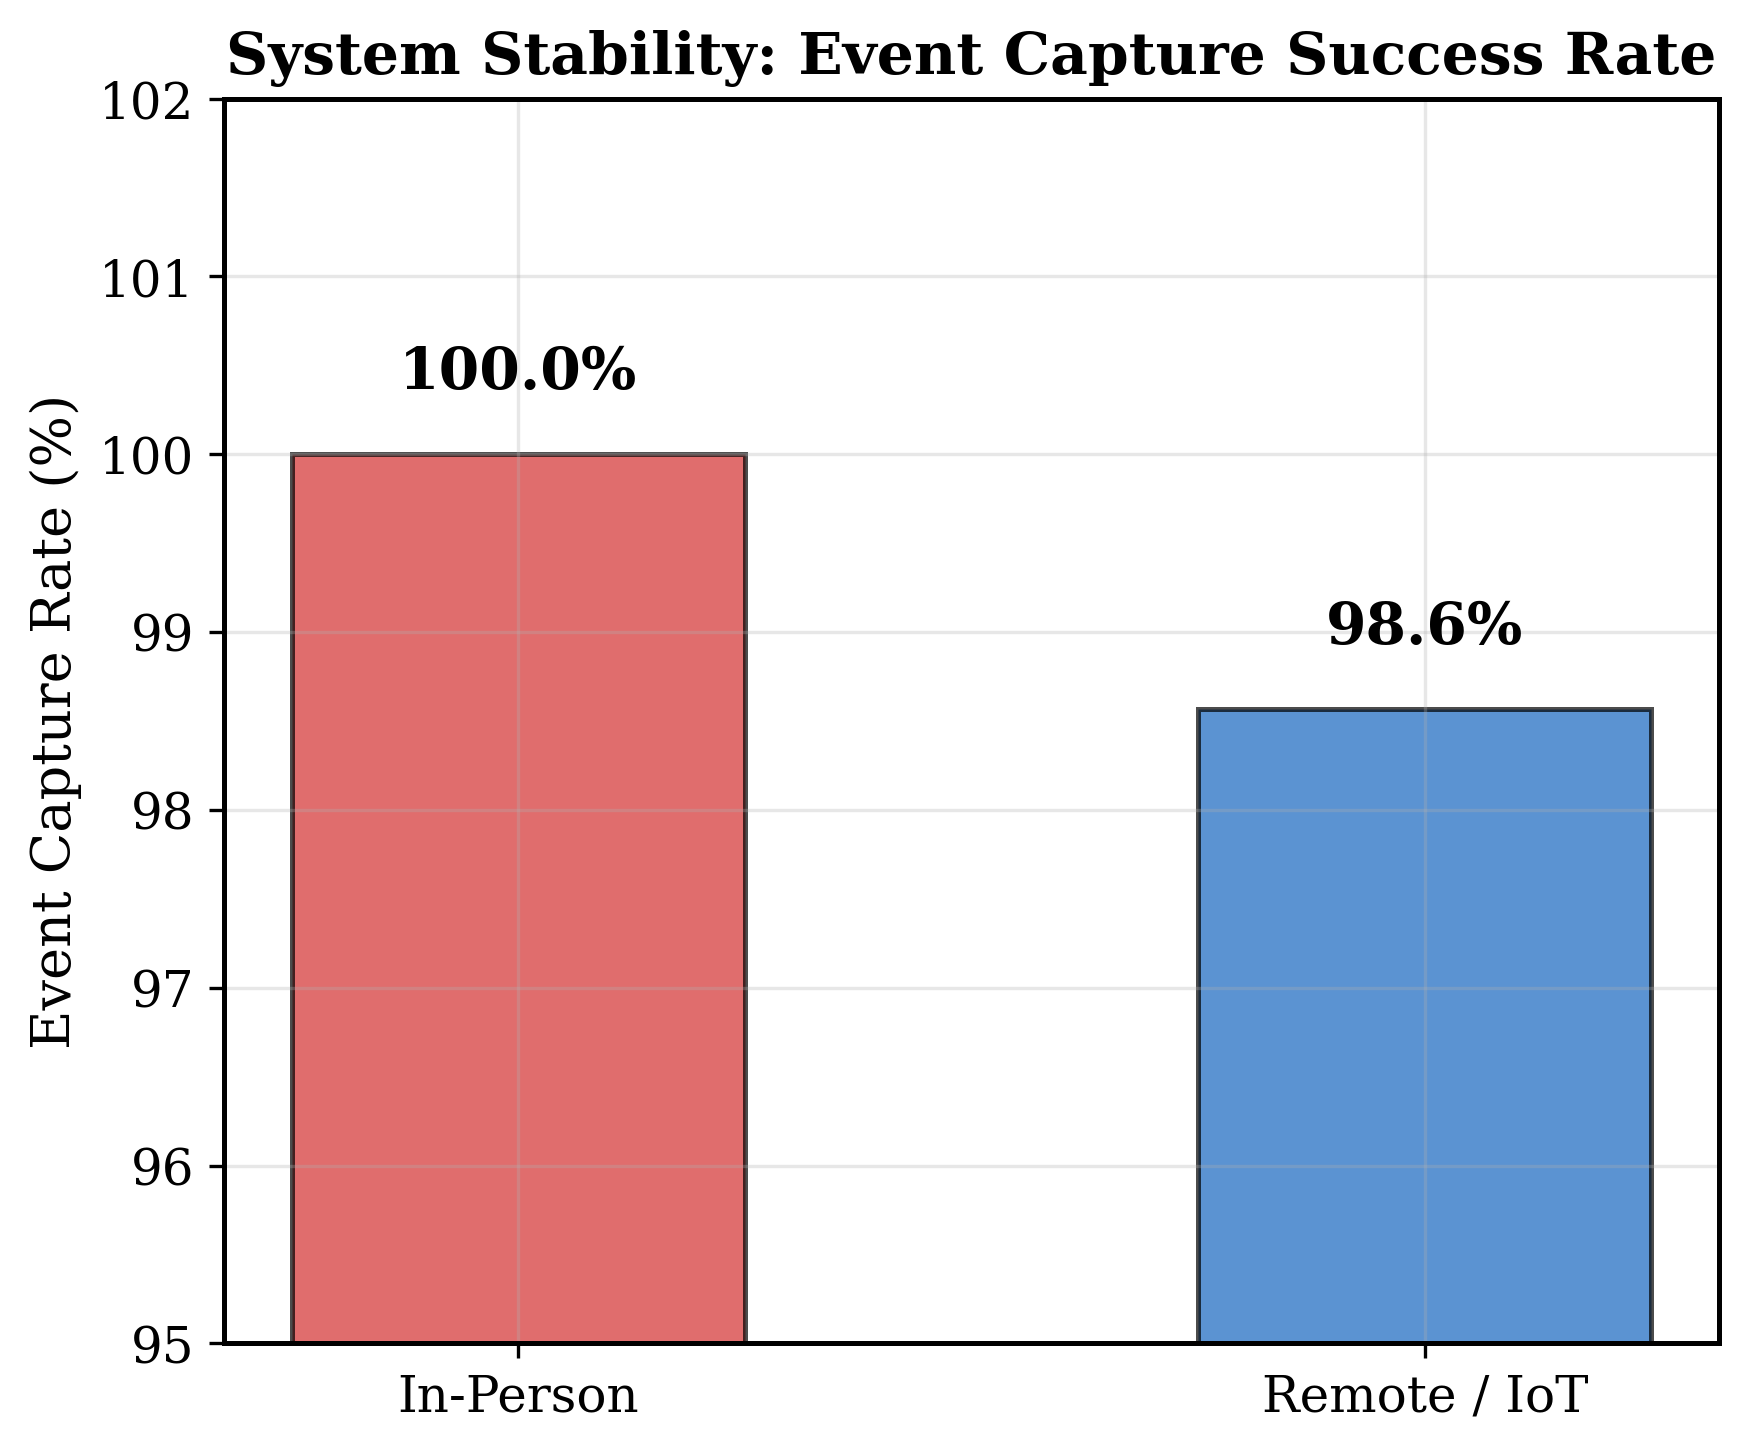
\includegraphics[width=\linewidth]{figures/stability_success_rate.png}
  \caption{Tasa de captura exitosa de eventos: remoto (98,5\%) vs. presencial (100,0\%).}
  \label{fig:stability}
\end{figure}

\subsection{Discusi\'on}

Los resultados obtenidos demuestran que el sistema de {\itshape retrofitting} IoT es capaz de capturar la din\'amica del experimento de MRUA con fidelidad comparable e incluso superior en estabilidad al montaje presencial tradicional. Contrariamente a las expectativas para sistemas distribuidos, las mediciones en modo remoto mostraron dispersi\'on controlada, evidenciando la eficiencia del manejo de interrupciones en el m\'odulo de control. La consistencia de los datos sugiere que la latencia de red, aunque presente, no degrad\'o la calidad de la recolecci\'on de datos cinem\'aticos gracias al estampado temporal local.

La viabilidad t\'ecnica del modelo propuesto tiene implicaciones directas para la modernizaci\'on de infraestructuras educativas con recursos limitados. El enfoque de \textit{retrofitting} demuestra que es posible transformar equipamiento cl\'asico en activos digitales conectados sin reemplazar la instrumentaci\'on original. La arquitectura modular adoptada permite una escalabilidad eficiente, donde la capa de sensado y control est\'a desacoplada de los servicios de visualizaci\'on y almacenamiento. Los resultados validan que las soluciones de bajo costo basadas en hardware de consumo masivo pueden alcanzar niveles de precisi\'on adecuados para prop\'ositos acad\'emicos, facilitando la transici\'on hacia entornos de aprendizaje h\'ibridos.

Los coeficientes de correlaci\'on de Pearson ($r \approx 0$) no deben interpretarse como una limitaci\'on del sistema IoT. Los valores son consistentes con lo esperado para series independientes no emparejadas que comparten la misma fuente de variabilidad f\'isica: la naturaleza estoc\'astica del lanzamiento manual del carrito introduce dispersi\'on id\'entica en ambas modalidades, lo que limita el coeficiente de correlaci\'on sin afectar la equivalencia de las distribuciones~\cite{giavarina2015}. El an\'alisis Bland--Altman (Tabla~\ref{tab:bland_altman}) confirma que los l\'imites de concordancia al 95\% son del orden de $\pm$0,5--0,8~s, consistentes con la variabilidad natural del MRUA, lo cual es t\'ecnicamente aceptable para el prop\'osito pedag\'ogico del experimento.

Al contrastar los resultados con la literatura previa, se observan similitudes fundamentales con los trabajos de Viswanadh \textit{et al.}~\cite{r2} y Lustig \textit{et al.}~\cite{r5} respecto a la efectividad de arquitecturas modulares para experimentos remotos. Sin embargo, el presente estudio aporta una validaci\'on cuantitativa espec\'ifica para el caso del MRUA. A diferencia de las soluciones basadas en SmartIPL revisadas por Zhao~\cite{r6}, que dependen de sensores internos del tel\'efono inteligente, el sistema implementado ofrece una infraestructura fija y dedicada que garantiza mayor repetibilidad manteniendo la accesibilidad econ\'omica.

La Tabla~\ref{tab:comparacion} presenta una comparaci\'on sistem\'atica con trabajos relacionados.

\begin{table*}[t]
\caption{Comparaci\'on sistem\'atica con trabajos relacionados.}
\label{tab:comparacion}
\centering
\scriptsize
\renewcommand{\arraystretch}{1.3}
\begin{tabular}{p{2.0cm}p{1.3cm}p{1.5cm}p{1.8cm}p{0.8cm}p{0.8cm}p{0.6cm}p{0.6cm}p{3.0cm}}
\toprule
\textbf{Trabajo} & \textbf{Estrategia} & \textbf{Hardware} & \textbf{Valid. remota} & \textbf{Costo} & \textbf{Rec. ltd.} & \textbf{Web} & \textbf{Abierto} & \textbf{Latencia} \\
\midrule
Este trabajo & Retrofitting & ESP32 + RPi~4 & S\'i (cuant.) & $<$150 & S\'i & S\'i & S\'i & Timestamp local \\
Lustig~\cite{r10} & Retrofitting & ESP32 + RPi & No & $\sim$200 & Parcial & S\'i & S\'i & $\approx$220\,ms \\
P\'erez-Cham\'e~\cite{r11} & Nuevo HW & ESP32 & No & $\sim$100 & S\'i & No & Parcial & NR \\
Guerrero-O.~\cite{r4} & Nuevo sist. & Arduino + nube & No & $>$500 & No & S\'i & No & NR \\
Viswanadh~\cite{r2} & Retrofitting & RPi + sensores & No & $\sim$200 & S\'i & Parcial & No & NR \\
Fuertes~\cite{r3} & Nuevo sist. & Embebido + nube & No & $>$500 & No & S\'i & No & NR \\
\bottomrule
\end{tabular}
\end{table*}

\subsection{Limitaciones}

El sistema depende de la disponibilidad continua del servidor MQTT. El n\'umero de ensayos ($n=35$ por modalidad) se limita a un entorno de laboratorio controlado. La fricci\'on residual del carrito y la alineaci\'on de los sensores introducen variaciones f\'isicas independientes de la instrumentaci\'on IoT.

%========================================================
\section{Conclusiones}

El sistema de \textit{retrofitting} IoT propuesto demostr\'o la capacidad de reproducir mediciones de MRUA con precisi\'on estad\'isticamente equivalente al montaje presencial de referencia. Las diferencias medias fueron inferiores a 0,03~s en todos los puntos de medici\'on, con $\Delta\sigma < 0{,}02$~s. El resultado m\'as significativo es la igualdad de la aceleraci\'on experimental media en ambas modalidades ($\mu \approx 0{,}95$~m/s$^2$, $n = 35$ cada una), con una desviaci\'on del 3,3\% respecto al valor te\'orico ($a \approx 0{,}92$~m/s$^2$). La tasa de captura exitosa de eventos fue del 98,5\% en modo remoto.

La contribuci\'on central es la validaci\'on cuantitativa de que un sistema IoT de bajo costo ($<$~USD~150) basado en Edge computing con ESP32 puede replicar las capacidades de medici\'on de un montaje presencial de cinem\'atica. La arquitectura de tres capas, con c\'odigo de fuente abierta en GitHub~\cite{r15}, es directamente replicable.

El estudio presenta tres limitaciones: (1)~la validaci\'on se limita a un \'unico experimento (MRUA); (2)~no se evaluaron indicadores de aprendizaje; (3)~la estabilidad depende de la calidad de la red WiFi.

Las l\'ineas de investigaci\'on futura prioritarias incluyen:
\begin{enumerate}
  \item Extensi\'on a otros experimentos de f\'isica: din\'amica, energ\'ia y ondas.
  \item Evaluaci\'on del aprendizaje con grupos reales de estudiantes.
  \item Integraci\'on con sistemas LMS (Moodle, Canvas).
  \item Sensores de mayor resoluci\'on temporal (fotopuertas $<$~1~ms).
  \item Implementaci\'on de QoS nivel~1 en MQTT para redes inestables.
\end{enumerate}

%========================================================

\section*{Agradecimientos}
El desarrollo y evaluaci\'on del prototipo se realizaron con la autorizaci\'on expl\'icita de la Pontificia Universidad Cat\'olica del Ecuador, sede Esmeraldas.
%========================================================

\bibliography{referencias_articulo.bib}
\bibliographystyle{IEEEtran}
\end{multicols}
\end{document}

